\documentclass{article}

\usepackage[english]{babel}
\usepackage[utf8]{inputenc}
\usepackage{amsmath,amssymb}
\usepackage{parskip}
\usepackage{graphicx}
\usepackage{listings}
\usepackage{float}

% Margins
\usepackage[top=2.5cm, left=3cm, right=3cm, bottom=4.0cm]{geometry}
% Colour table cells
\usepackage[table]{xcolor}
\lstset{
    numbers=left, 
    numberstyle= \tiny, 
    keywordstyle= \color{ blue!70},
    commentstyle= \color{red!50!green!50!blue!50}, 
    frame=shadowbox, % 阴影效果
    rulesepcolor= \color{ red!20!green!20!blue!20} ,
    escapeinside=``, % 英文分号中可写入中文
    xleftmargin=2em,xrightmargin=2em, aboveskip=1em,
    framexleftmargin=2em,
    breaklines=true,
    language=python
} 

% Get larger line spacing in table
\newcommand{\tablespace}{\\[1.25mm]}
\newcommand\Tstrut{\rule{0pt}{2.6ex}}         % = `top' strut
\newcommand\tstrut{\rule{0pt}{2.0ex}}         % = `top' strut
\newcommand\Bstrut{\rule[-0.9ex]{0pt}{0pt}}   % = `bottom' strut

%%%%%%%%%%%%%%%%%
%     Title     %
%%%%%%%%%%%%%%%%%
\title{CSCI803 Assignment}
\author{Yao Xiao \\ SID 2019180015}
\date{\today}

\begin{document}
\maketitle

%%%%%%%%%%%%%%%%%
%   Problem 1   %
%%%%%%%%%%%%%%%%%
\section{Problem 1}
\begin{equation*}
    A={
    \left[ \begin{array}{cccc}
    2 & 3 & 12 & 14\\
    4 & 8 & 16 & \infty\\
    5 & 9 & \infty & \infty\\
    \infty & \infty & \infty & \infty
    \end{array} 
    \right ]}
\end{equation*}

\section{Problem 2}
For the first question, if the first element is $\infty$, the rest of the first row need to be $\infty$.
In this case, all other elements need to be $\infty$ because they are larger than the first element on their column.

For the second question, if the bottom right element is smaller than $\infty$, all the elements on the bottom row need to be smaller than $\infty$.
So, the other elements, each of them must be smaller than the bottom element on its column.

\section{Problem 3}
Actually, we can execute a processs (similar to MAXHEAPIFY) to restore.

For $A[i,j]$, we can compare it with each of its neighbours and exchange it with the smallest.
And this does not destroy and will restore the property of $A[i,j]$, but this will simplify the problem to both
$A[i+1, j]$ and $A[i, j+1]$.

When $A[i, j]$ is smaller than its neighbours, the processs will be terminated.

The relation is: 

\begin{equation}
\begin{aligned}
    T(p) &= T(p-1) + O(1)\\
    &= T(p-2) + O(1) + O(1)\\
    &= T(p-3) + O(1) + O(1) + O(1)\\
    &= \cdots\\
    &= O(p)
\end{aligned}
\end{equation}

Here is the code:
\begin{lstlisting}
    def res_tableau(tableau, i=0, j=0):

    bottom = tableau[i + 1][j] if (i + 1 < m) else float('inf')
    right = tableau[i][j + 1] if (j + 1 < n) else float('inf')

    if bottom < right:

        temp = tableau[i][j]
        tableau[i][j] = tableau[i + 1][j]
        tableau[i + 1][j] = temp

        res_tableau(tableau, i + 1, j)

    if bottom > right:

        temp = tableau[i][j]
        tableau[i][j] = tableau[i][j + 1]
        tableau[i][j + 1] = temp

        res_tableau(tableau, i, j + 1)


def extract_min(tableau):

    min = tableau[0][0]

    tableau[0][0] = float('inf')

    res_tableau(tableau)

    return min


tableau = [[10, 12, 15, 17], [11, 18, 20, 25], [22, 27, 30, 35],
           [34, 40, 44, 88]]

(m, n) = (len(tableau), len(tableau[0]))

for i in range(m * n):
    print(extract_min(tableau))

\end{lstlisting}

\textbf{Output:}
\begin{figure}[H]
    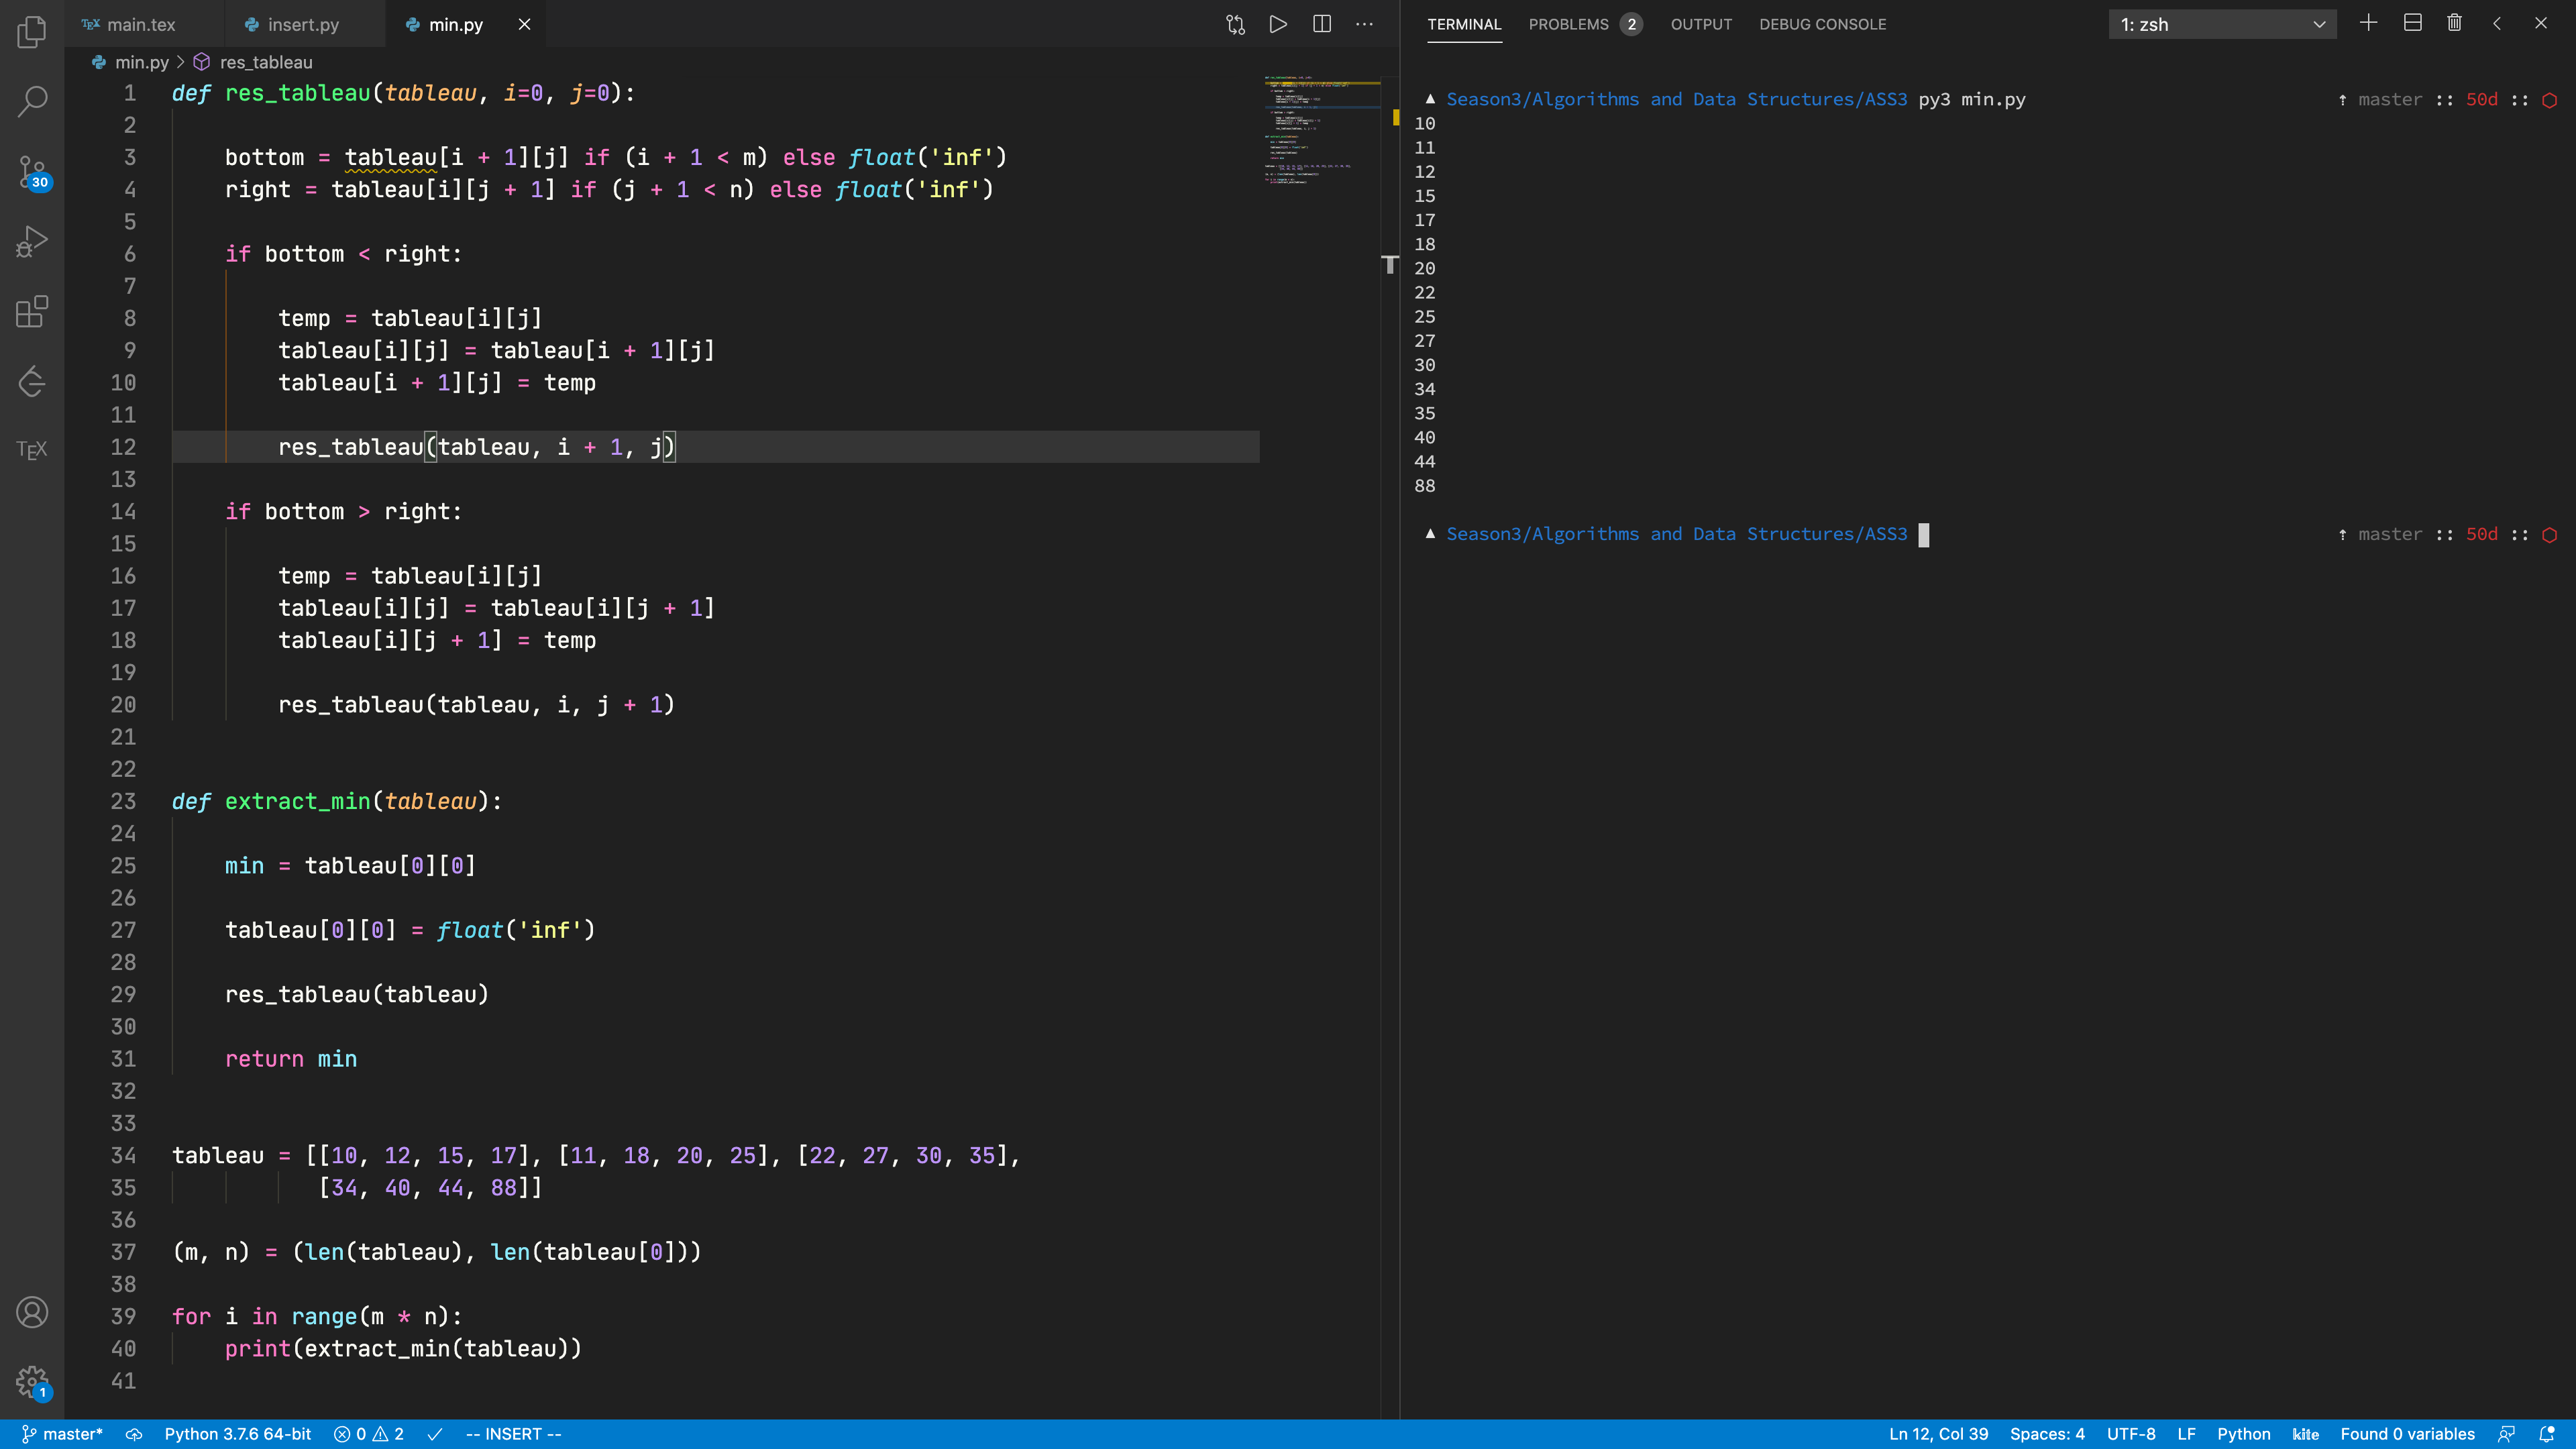
\includegraphics[width=1\textwidth]{Fig2}
\end{figure}

\section{Problem 4}
In fact, the algorithm is similar as the previous.
However, the difference is that we need to start with the bottom right element of the table, and then move it upwards and leftwards to the correct position.

For example, assuming that we have inserted the element into the bottom right of the matrix, now we need to move it to a suitable position in the matrix. If it has elements on the top and left, then choose the largest one to exchange with it; if it doesn’t have values on both the top and left, then choose to move up or move to the left first. Considering the characteristics of matrix storage, it is better to move up first.

Even if we have an empty array and are inserting new elements, these elements will only be traversed (i+j). The maximum values of i and j are m and n, so the running time is O(m + n).

Here is the code:
\begin{lstlisting}
def insert(tableau, i, j):
    if i == 0 and j == 0:
        return

    if i == 0:
        if tableau[i][j] < tableau[i][j - 1]:
            temp = tableau[i][j]
            tableau[i][j] = tableau[i][j - 1]
            tableau[i][j - 1] = temp

            insert(tableau, i, j - 1)
        return

    if j == 0:
        if tableau[i][j] < tableau[i - 1][j]:

            temp = tableau[i][j]
            tableau[i][j] = tableau[i - 1][j]
            tableau[i - 1][j] = temp
            insert(tableau, i - 1, j)
        return

    if tableau[i][j] < tableau[i - 1][j]:
        temp = tableau[i][j]
        tableau[i][j] = tableau[i - 1][j]
        tableau[i - 1][j] = temp

        insert(tableau, i - 1, j)

    if tableau[i][j] < tableau[i][j - 1]:
        temp = tableau[i][j]
        tableau[i][j] = tableau[i][j - 1]
        tableau[i][j - 1] = temp

        insert(tableau, i, j - 1)


def print_tableau(tableau):

    for i in range(M):
        for j in range(N):
            print(tableau[i][j], end=' ')
        print()


def insert_keys(tableau, keys):

    for key in keys:
        if tableau[M - 1][N - 1] != float('inf'):
            print("Full! Skip key:", key)
        else:
            tableau[M - 1][N - 1] = key

            insert(tableau, M - 1, N - 1)


M = N = 4

tableau = [[float('inf') for x in range(N)] for y in range(M)]

keys = [12, 8, 20, 22, 25, 32, 34, 11, 43, 27, 16, 40, 88, 15, 18, 45]

insert_keys(tableau, keys)
print_tableau(tableau)
\end{lstlisting}

\textbf{Output:}
\begin{figure}[H]
    \centering
    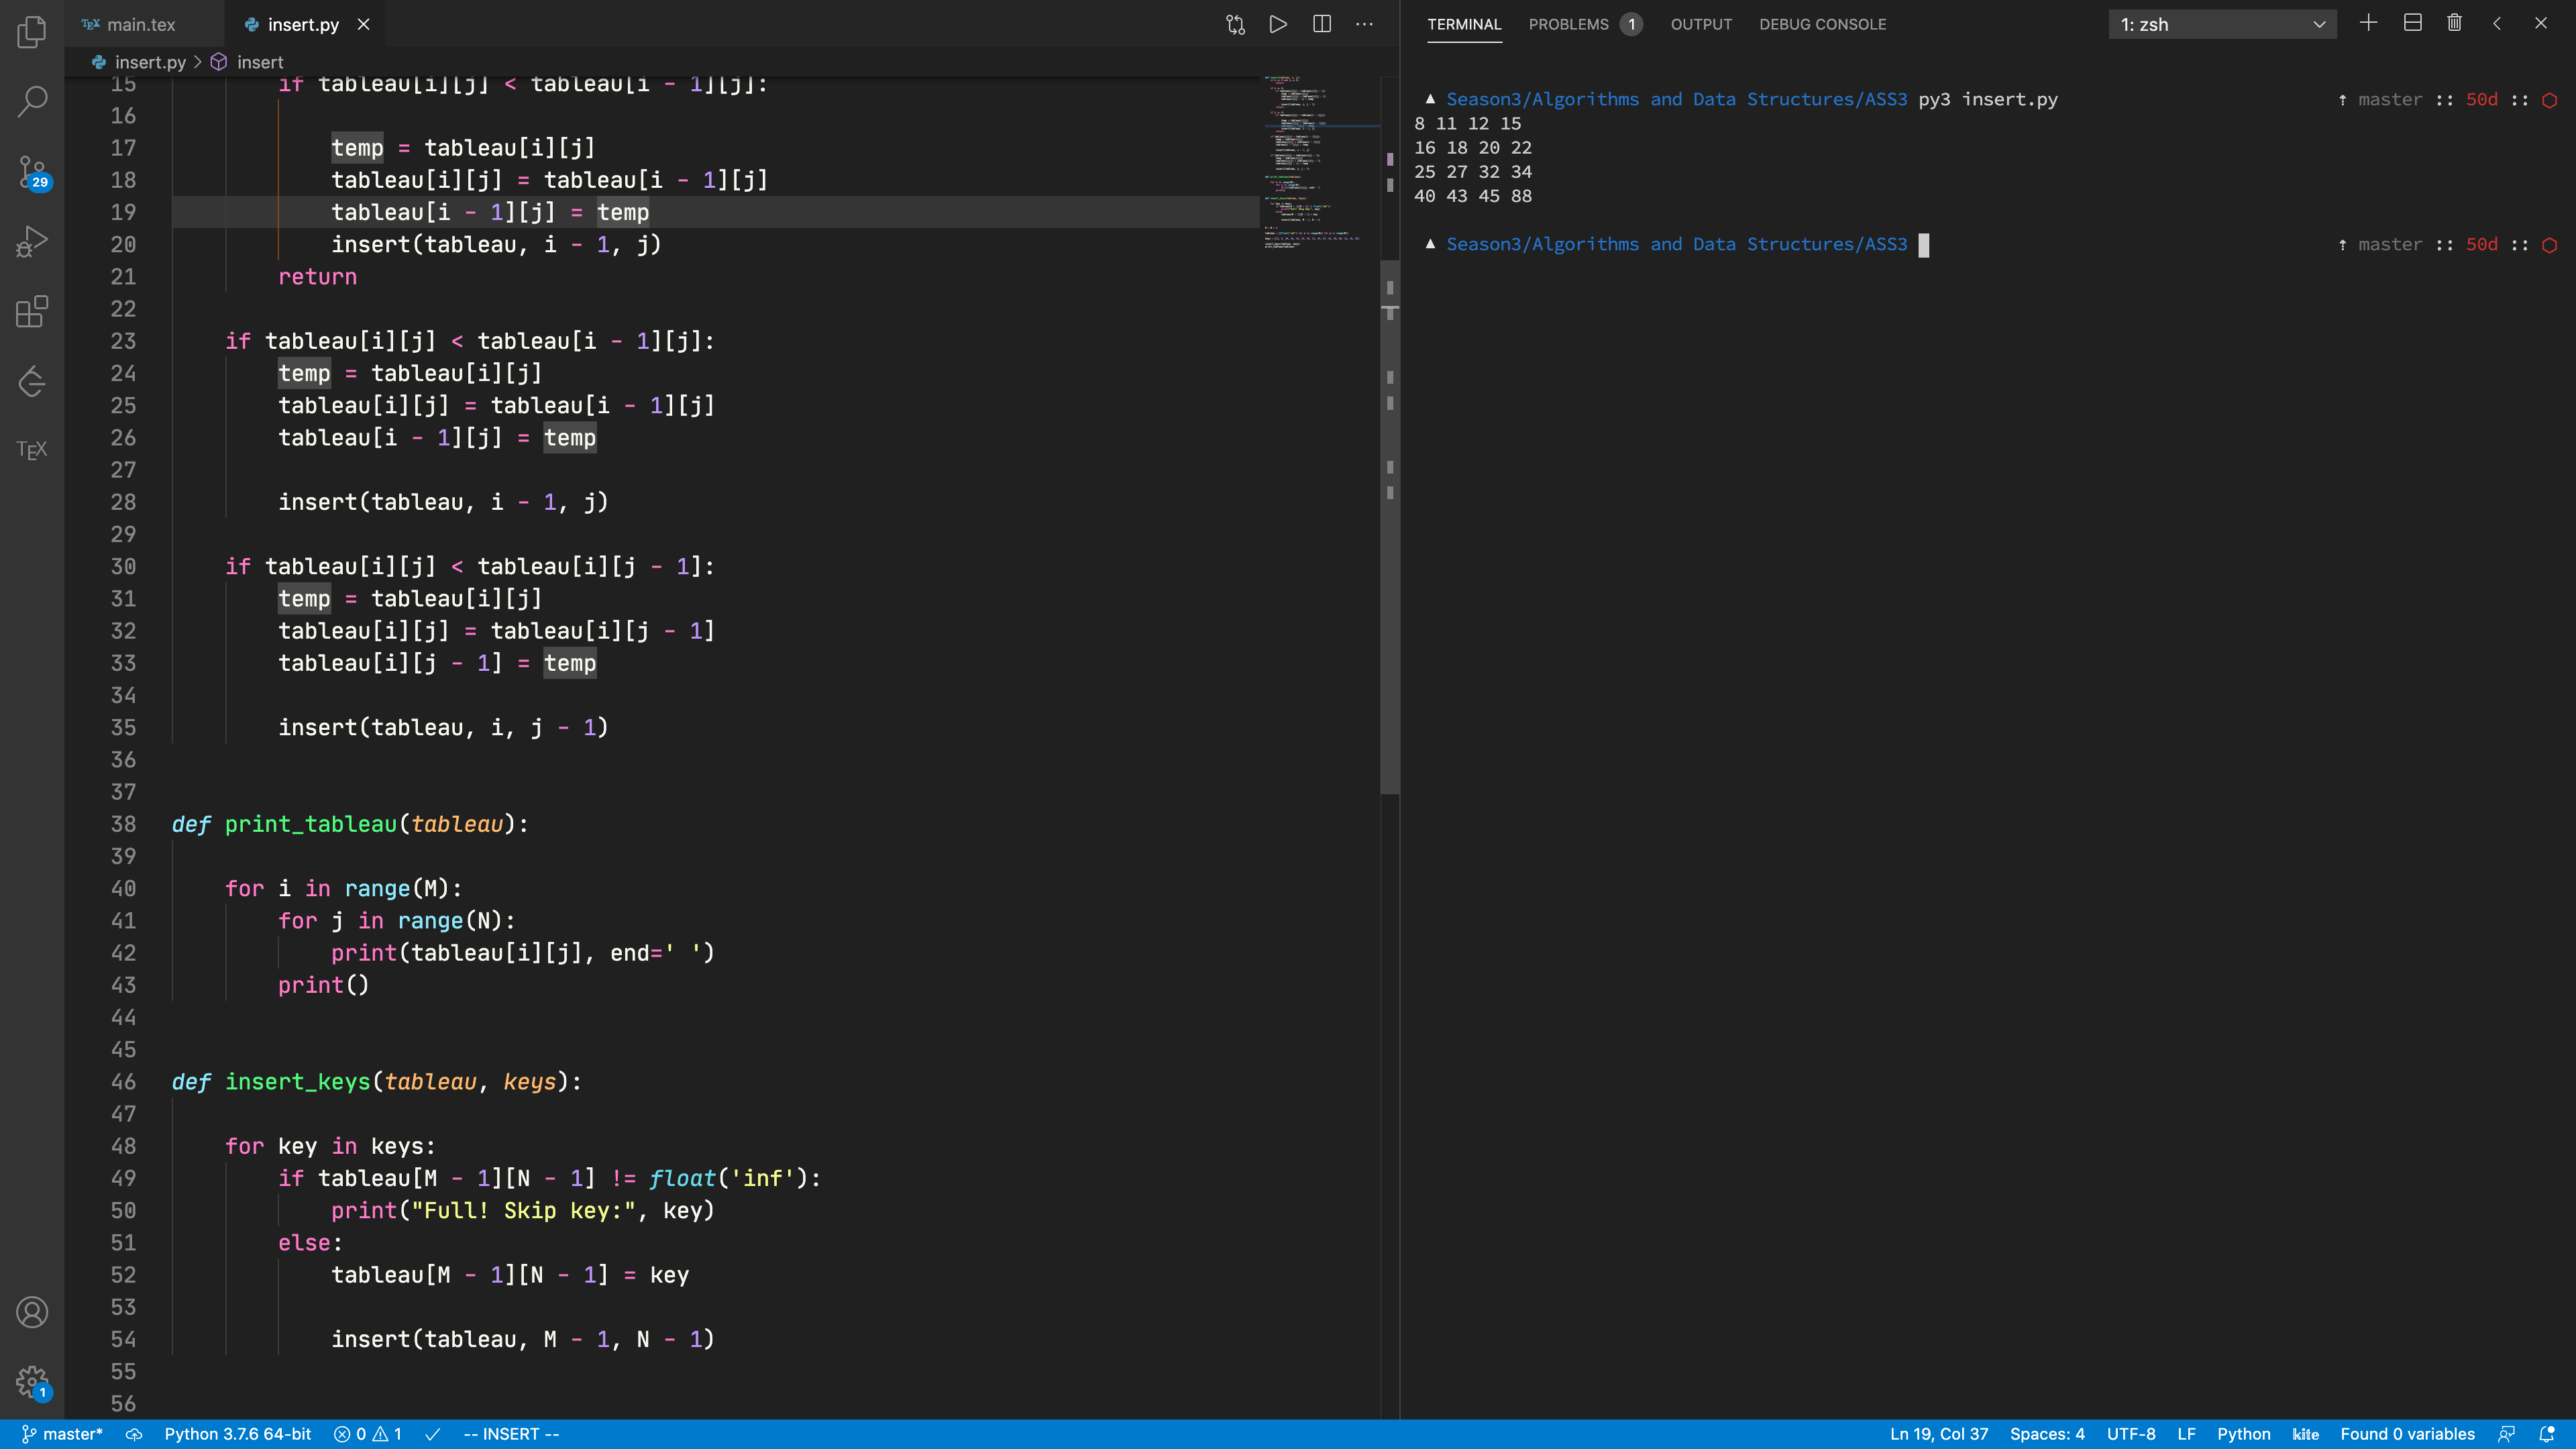
\includegraphics[width=1\textwidth]{Fig1}
\end{figure}

\section{Problem 5}
Here is the pseudocode $\textbf{sort(A)}$:
\begin{lstlisting}
for i = 1 to m
insert(Y,n,n,A[i])
for i = 1 to m
A[i] = EXTRACT-MIN(Y)
\end{lstlisting}

We can sort by starting with an empty tableau and inserting all the $n^2$ elements in it,
line 1 to 2 is inserting $n^2$ in to tableau which takes O(n+n) and lines 3 to 4 extract $n^2$ and EXTRACT-MIN runs O(n+n),
so this gives the running time of $n^2O(n) = O(n^3)$.

\section{Problem 6}
\begin{lstlisting}
def search(tableau, key):

    i = 0
    j = len(tableau[0]) - 1

    while i < len(tableau) and j >= 0:

        if tableau[i][j] < key:
            i = i + 1

        elif tableau[i][j] > key:
            j = j - 1

        else:
            return True

    return False


tableau = [[10, 12, 15, 17], [11, 18, 20, 25], [22, 27, 30, 35],
           [34, 40, 44, 88]]


keys = [8, 17, 26, 88]

for key in keys:
    if search(tableau, key):
        print("Key", key, "found in table!")
    else:
        print("Error: No element found!")
\end{lstlisting}

\textbf{Output:}
\begin{figure}[H]
    \centering
    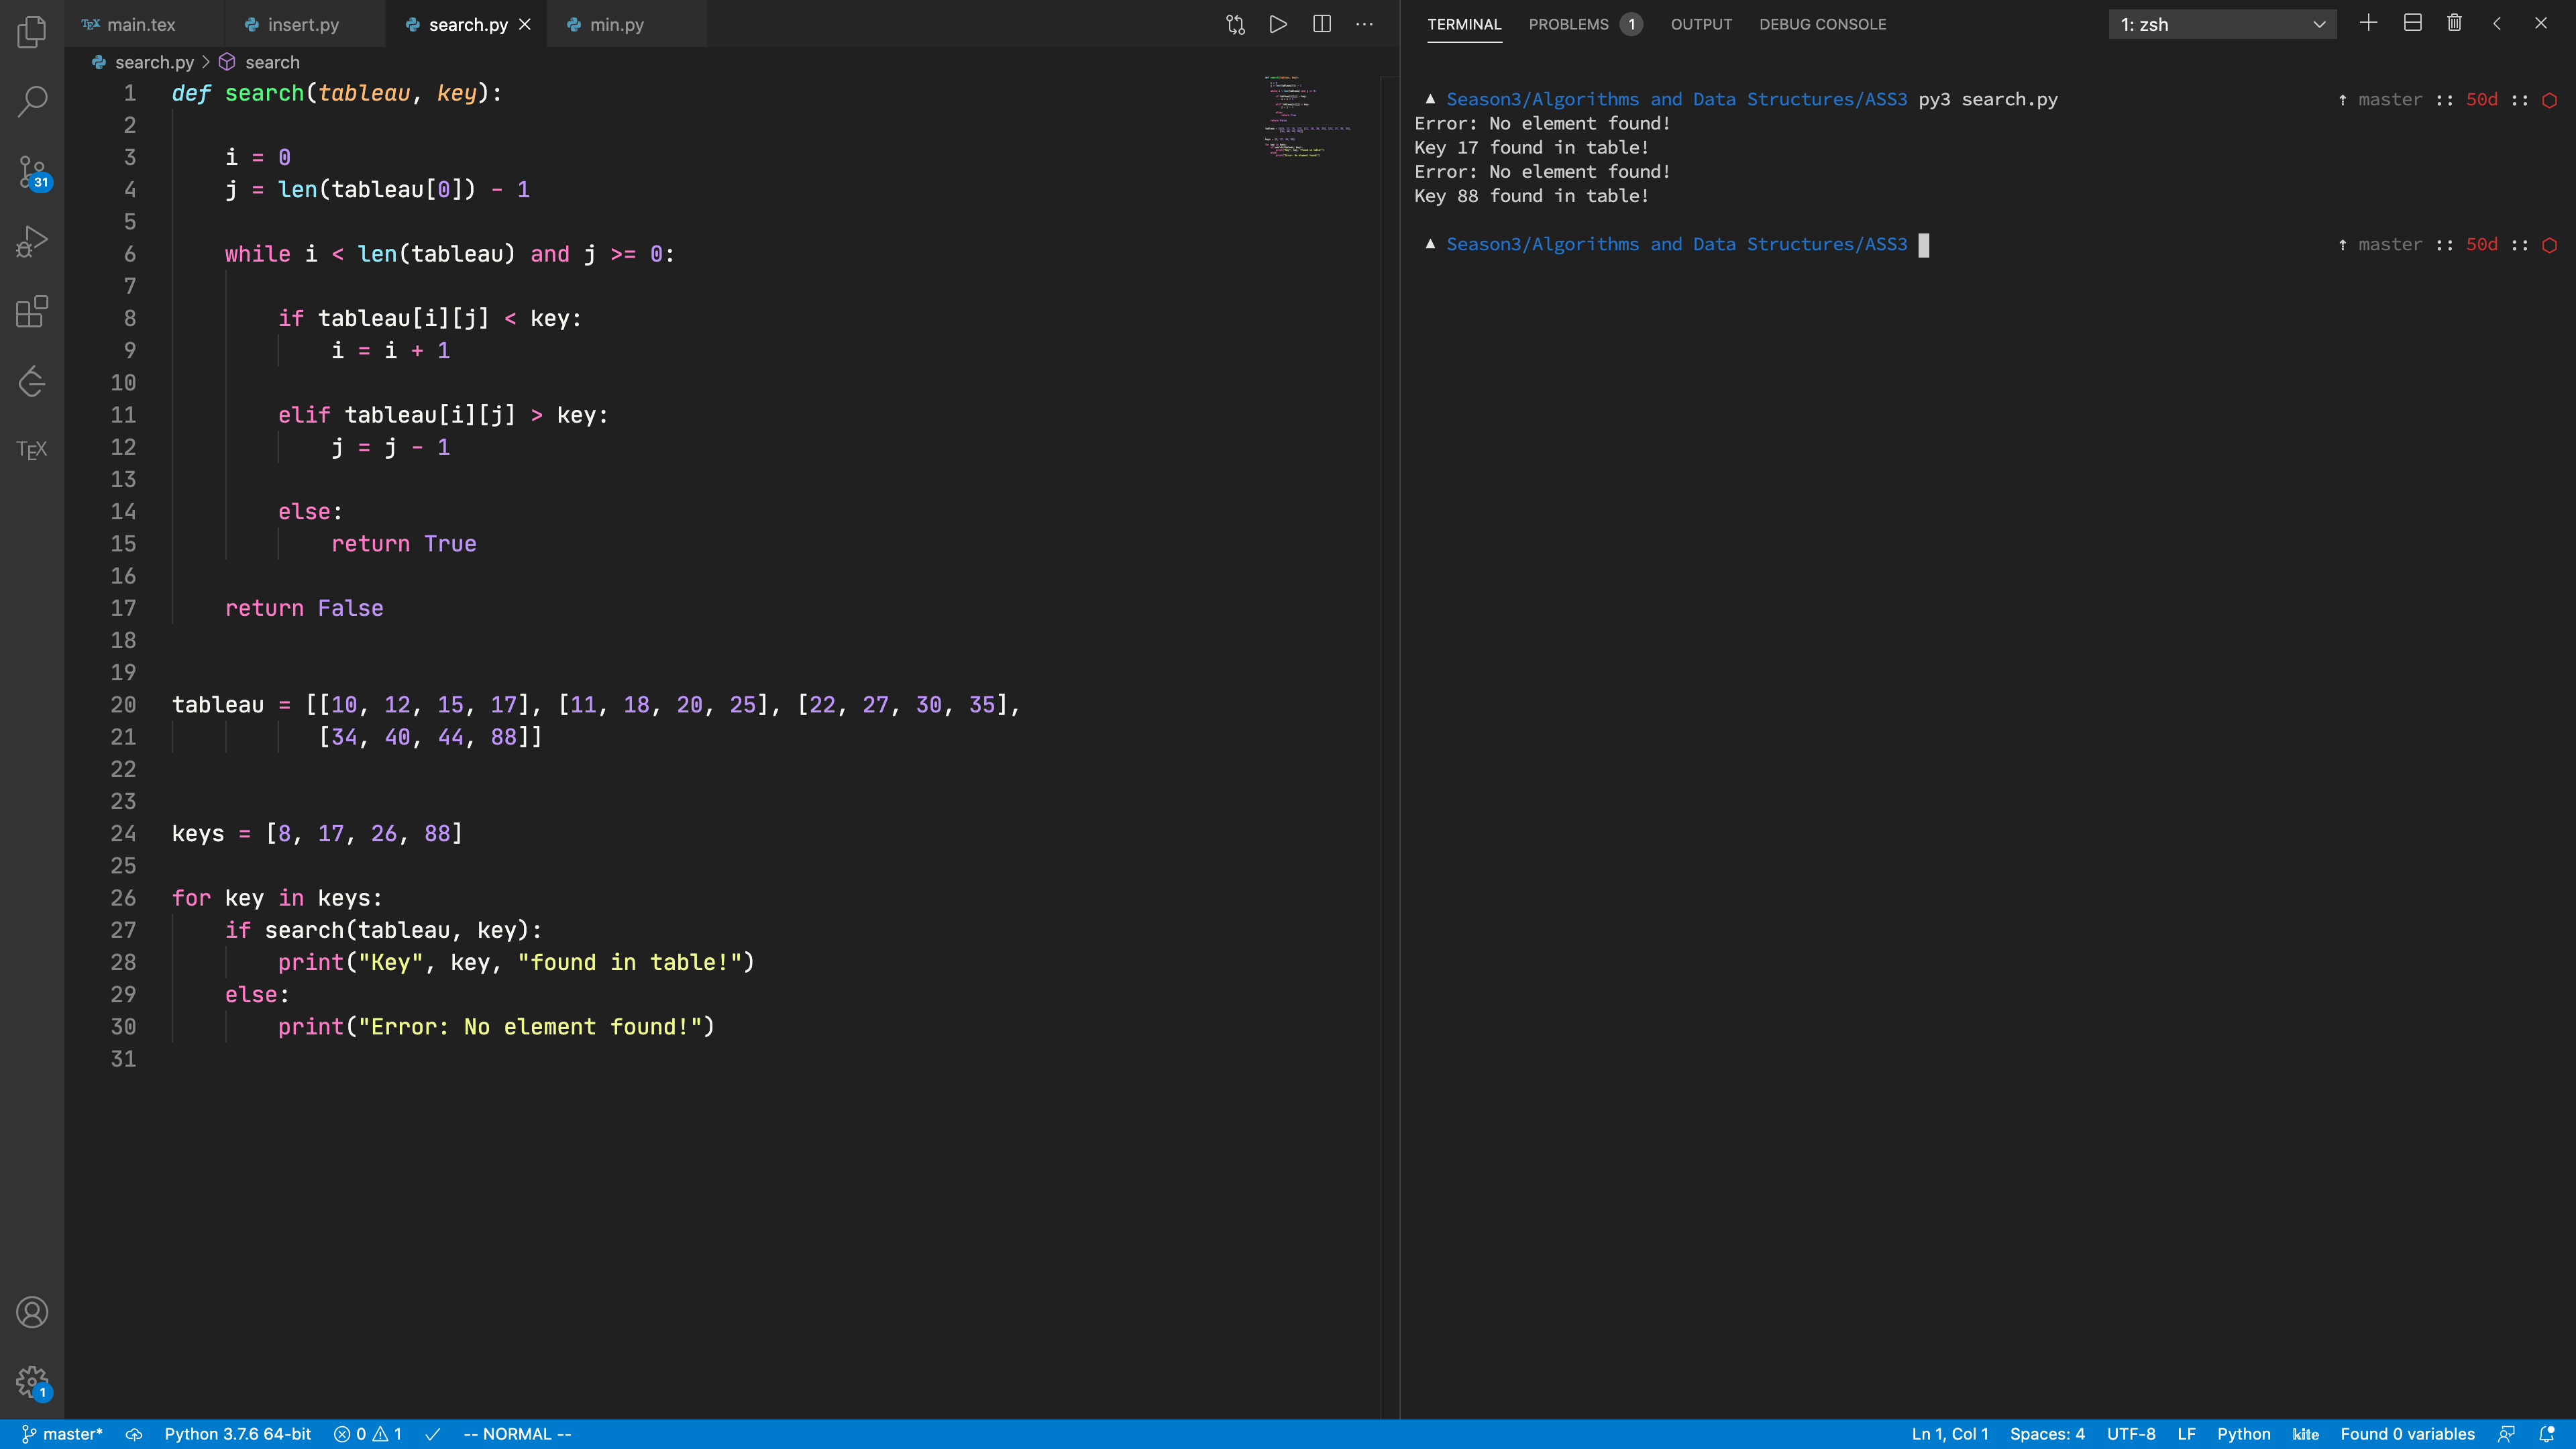
\includegraphics[width=1\textwidth]{Fig3}
\end{figure}


\end{document}

